\documentclass[10pt,aspectratio=169]{beamer}

% All the boilerplate is in ccaslides.sty
% Note that this also pulls in a custom vogtwidebar.sty
\usepackage{ccaslides}

\author{Ji\v{r}\'i Lebl}

\institute[OSU]{%
Departemento pri Matematiko de Oklahoma {\^S}tata Universitato}

\title{Cultivating Complex Analysis:\\%
The logarithm (4.1.1)}

\date{}

\begin{document}

\begin{frame}
\titlepage
\end{frame}

\begin{frame}
Consider the primitive of $z^n$.

\medskip
\pause

If $n\not=-1$, then the primitive is 
$\dfrac{z^{n+1}}{n+1}$ (not defined at the origin if $n+1 < 0$)

\medskip
\pause

What about $z^{-1} = \nicefrac{1}{z}$?

\medskip
\pause

Consider the \emph{slit plane}
\[
U = \C \setminus (-\infty,0] = \C \setminus \bigl\{ z \in \C : \Re z \leq 0 , \Im z = 0 \bigr\}.
\]

\pause

$U$ is star-shaped $\Rightarrow$ holomorphic functions on $U$ have a primitive on
$U$, including $\nicefrac{1}{z}$.

\medskip
\pause

Require this primitive to be $0$ at $z=1$ to obtain
the \emph{principal branch} of the logarithm:
\[
\operatorname{Log} \colon U \to \C 
\]
\pause
We wish to show that Log is equal to
$\log \sabs{z} + i \Arg z$ (principal branch of the argument).
\end{frame}

\begin{frame}
Set $L(z) = \log \sabs{z} + i \Arg z$ \qquad (WTS that $L = \Log$).

\medskip
\pause

$L(1) = 0 = \Log(1)$, good!

\medskip
\pause

$
e^{L(z)}
=
e^{\log \sabs{z}} e^{i \Arg z}
=
\sabs{z} e^{i \Arg z} = z .
$

\pause
\medskip

So $L$ is the inverse of the exponential, so holomorphic.

\medskip
\pause
Differentiate $z = e^{L(z)}$:
\qquad
\pause
$
1 = L'(z) e^{L(z)} = L'(z) z .
$

\medskip
\pause
Et voil\`a!

\medskip
\pause

Using a different branch of the argument gets another antiderivative.

\medskip
\pause

Emboldened, we define
\[
\log z \overset{\text{def}}{=} \log \sabs{z} + i \arg z .
\]
\pause
That sounds crazy: \pause

1) The $\log$ on the right (the real log) is different than the $\log$ on
the left, and

\pause
2) $\arg$ has infinitely many values.
\end{frame}

\begin{frame}
Here are the real and imaginary parts of
$\log z = \log \sabs{z} + i \arg z$:

\medskip

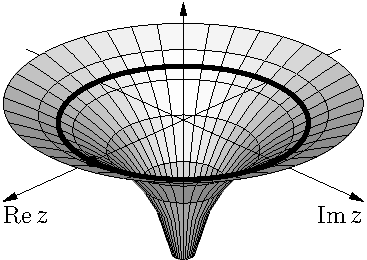
\includegraphics{../figures/logrealgraph}
\qquad
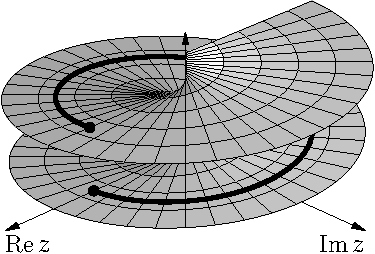
\includegraphics{../figures/arggraph2}

\pause
\medskip

If we travel the unit circle in the $z$-plane, we travel the
marked path on the graph.

\medskip
\pause

The real part is a nice function, it is the normal real $\log \colon
(0,\infty) \to \R$ applied to $\sabs{z}$.

\medskip
\pause

The imaginary part has infinitely many values.

\medskip
\pause

Nevertheless, it is the correct definition.  Much more useful than the principal branch.
\end{frame}

\begin{frame}
How do we use $\log$?  To compute line integrals:

\medskip
\pause

Parametrize $\partial \D$ starting and ending at $z=1$ and compute:
\[
\int_{\partial \D} \frac{1}{z} \, dz
\pause
= \log 1 - \log 1
\pause
= 2\pi i.
\]

\pause
That's nonsense!  Let's make it better:
\pause
\[
\int_{\partial \D} \frac{1}{z} \, dz
\enspace
\text{``$=$''}
\enspace
\log 1 - \log 1
\enspace
\text{``$=$''}
\enspace
2\pi i.
\]

\pause

Maybe still not quite right.

\medskip
\pause

It works by following one ``branch'' of the logarithm along the path
and then subtracting.

\medskip
\pause

Let's see that graph again.
\end{frame}

\begin{frame}
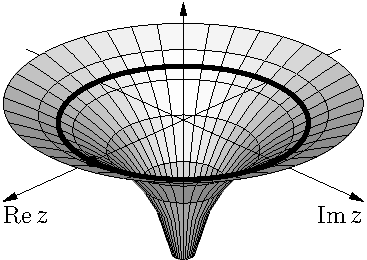
\includegraphics{../figures/logrealgraph}
\qquad
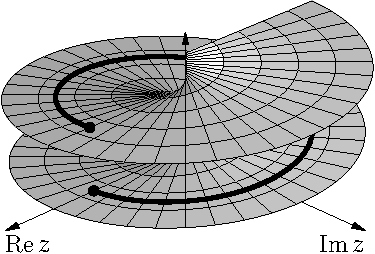
\includegraphics{../figures/arggraph2}

\pause
\medskip

What we do:

\medskip
\pause

We start with the value $\log 1 = 0$.

\medskip
\pause

Then we follow the graph around the circle until we end at
$\log 1 = 2\pi i$.
\end{frame}

\begin{frame}
A \emph{branch} of the logarithm in $U$ is an antiderivative of
$\nicefrac{1}{z}$ in $U$ that equals one value of $\log z$ at every point.

\medskip
\pause

We say we \emph{follow a branch} along a path by taking a branch in some
small neighborhood,

\pause

then change to another branch in another small
neighborhood (equal at some point). \pause Etc.

\medskip
\pause

\begin{center}
\subimport*{../figures/}{followbranch.pdf_t}
\end{center}

\medskip
\pause

That's what we did in the computation above.
\end{frame}

\end{document}
